\documentclass[twoside, letterpaper]{report}

% \usepackage{showframe}
\usepackage{graphicx}
\usepackage{geometry}
\usepackage{titlesec}
\usepackage{tabularx}
\usepackage{indentfirst}
\usepackage{pifont}
\usepackage[english]{babel}
\usepackage[twoside]{fancyhdr}
\usepackage[skip=10pt, indent=20pt]{parskip}
\usepackage{tikz}
\usetikzlibrary{positioning, shapes.geometric, shapes.misc}

\geometry{
top = 0.75in,
bottom = 0.75in,
outer = 0.75in,
inner = 1.5in,
}
\textheight = 8.5in

\pretolerance=5000
\tolerance=5000
\emergencystretch=10pt
\righthyphenmin=4
\lefthyphenmin=4

\newcommand{\cmark}{\centering \ding{51}}%
\newcommand{\xmark}{\centering \ding{55}}%

\renewcommand{\thispagestyle}[1]{} 
\renewcommand{\headrulewidth}{0pt}
\renewcommand{\footrulewidth}{0pt}

\titleformat{\chapter}[display]
    {\centering\Large\bf\vspace{-2cm}}{Chapter \thechapter}{0ex}{\Large}

\titleformat{\section}[display]
    {\bf}{}{0ex}{}
    
\setlength{\headheight}{75pt}
\headsep = 10pt

\fancyhf{} 
\fancyhead[C]{\raisebox{1cm}{\parbox{\headwidth}{\centering \textbf{\large WESTERN INSTITUTE OF TECHNOLOGY} \\ \textbf{La Paz, Iloilo City} \\ \underline{COLLEGE OF ENGINEERING} \\ DEPARTMENT OF COMPUTER ENGINEERING}}} 
\fancyhead[L]{
\includegraphics[width=2.5cm]{assets/WIT_logo.png}}
\fancyhead[R]{\raisebox{0.5cm}{
\includegraphics[width=3cm]{assets/GCL.jpg}}}

\title{\vspace{-3cm} MODULAR SELF-NAVIGATING UNMANNED SURFACE DRONE FOR MARINE APPLICATIONS\\}

\author{\vspace{1cm} \\ A Research Paper \\ Presented to \\ The Faculty of the Department of Computer Engineering
\\ Western Institute of Technology \\ Lapaz, Iloilo \vspace{2cm}
\\ In partial fulfillment of the requirements for the degree of \\ Bachelor of Science in Computer Engineering
\vspace{2cm} \\ By: \\ \\ Balasabas, Joseph \\ Cordero, John Angelo \\ Mondragon, John Gee \\ Pastrana, Jericho \vspace{2cm}} 
\date{April 2024}

\pagestyle{fancy}

\begin{document}

\maketitle

\setcounter{page}{1}

\chapter*{APPROVAL SHEET}
\setcounter{page}{1}

\chapter*{ACKNOWLEDGEMENT}
\setcounter{page}{1}

\chapter*{ABSTRACT}

\vspace{-1cm}
\begin{tabularx}{0.95\linewidth}{@{}p{0.45\linewidth}p{0.50\linewidth}@{}@{}}
\Large {\bf NAME OF INSTITUTION} & \Large Western Institute of Technology \\
\\
\Large {\bf ADDRESS} & \Large Luna Street La Paz, Iloilo \\
\\
\Large{\bf TITLE} & \Large Modular self-navigating unmanned surface drone for marine applications \\
\\
\Large {\bf AUTHOR} & \Large Balasabas, Joseph \\
 & \Large Cordero, John Angelo \\ 
 & \Large Mondragon, John Gee \\
 & \Large Pastrana, Jericho \\
\\
\Large {\bf TYPE OF DOCUMENT} & \Large Research Paper \\
\\
\Large {\bf DATE STARTED} & \Large todo \\
\\
\Large {\bf DATE COMPLETED} & \Large April 2024

\end{tabularx}


\Large The project is motivated by the desire to explore the potential benefits of modularity coupled with autonomy. Developing a water surface 
drone leveraging an ESP-32 microcontroller and incorporating autonomous navigation powered by GPS and magnetometer sensors to create an easy
to use and modular system by minimizing complexities, ensuring smooth operation and simplified troubleshooting. Testing procedures will 
evaluate the drone's accuracy in reaching designated target positions, providing quantitative insights into its navigational reliability. 
This project includes information on how to create said drone allowing anyone to reproduce it and use the drone as they see fit as it is 
modular by nature, some parts can be replaced or swapped out or even add new components to fit users intended use. Given the correct 
components, mapping lakes and rivers or monitoring ocean conditions for scientific research becomes a much easier task.

\setcounter{page}{1}
\tableofcontents
\clearpage

\fancyfoot[C]{\thepage}
\pagenumbering{arabic}
\chapter{Introduction}

\vspace{-1cm}

\paragraph{} This chapter has seven parts: (1) Background of the Study, (2) Statements of the Problem, (3) Theoratical Framework, 
            (4) Conceptual Framework, (5) Scope and Limitations, (6) Significance of the Study, and (7) Definition of Terms.

\paragraph{} Part one, Background of the Study, gives an overview as to which the research problem was anchored.

\paragraph{} Part two, Statement of the Problem, identifies the main problem and enumerates the specific problems which the study hoped to answer.

\paragraph{} Part three, Theoretical Framework, discussed the relevance of the variables in the identified theory, concept or principle to 
            the research problem.

\paragraph{} Part four, Conceptual Framework, presents the paradigm of the study.

\paragraph{} Part five, Scope and Limitations, specifies the scope and coverage of the study in terms of purpose, research design, 
            research instruments and statistical tools employed in the study.

\paragraph{} Part six, Significance of the Study, presents the possible contributions and the specific application of knowledge that 
            might be gained from the result of the study.

\paragraph{} Part seven, Definition of Terms, contains the conceptual and operational definitions of key terms used in the study.

\section{Background of the Study}
\paragraph{} As the ocean covers over 70\% of the Earth's surface, presenting a vast and complex environment ripe for exploration and study. 
            Sea surface drones offer a valuable tool for navigating water bodies, collecting data, and conducting research across various disciplines. 
            Unmanned surface vehicles (USVs) equipped with autonomous navigation capabilities have become pivotal in various applications, particularly 
            in water environments.

\paragraph{} Early USVs were also called ASC; Autonomous Surface Craft (ASCs) which were first developed at the MIT Sea Grant College Program in 1993 and 
            were designed for various missions. Aptly named ARTEMIS,the vessel was a scale replica of a fishing trawler used as a platform capable of 
            testing the navigation and control systems required by an ASC. Later on a new ASC ACES(Autonomous Coastal Exploration System) was developed 
            during 1996 and 1997(Justin E. Manley 2008)

\paragraph{} Further adaptation of USV in the early 20th century saw the development of remotely controlled USVs used for mine detection and target 
            practice. World War II further spurred advancements, with nations utilizing USVs for reconnaissance and explosive delivery. Post-war, 
            oceanographic research embraced USVs for data collection and underwater exploration. Notably, the bathyscaphe Trieste, equipped with a 
            rudimentary autopilot, famously reached the deepest point in the Earth's oceans in 1960( National Museum of the U.S. Navy)
          
\paragraph{} The 1990s witnessed a surge in commercial applications, with USVs employed for offshore oil and gas exploration, pipeline inspections, and 
            aquaculture monitoring. The 21st century has seen a continued proliferation of USVs, with advancements in sensor technology, autonomous 
            navigation systems, and communication capabilities propelling their capabilities further.

\paragraph{} However, while traditional methods for marine data collection involve time-consuming, expensive, and potentially risky manual operations,
            unmanned surface vehicles (USVs) offer a compelling alternative. These vehicles promise efficient, cost-effective, and safe data collection 
            across vast areas. However, current USV technology faces three key hurdles: high cost due to complex hardware and software, limited 
            accessibility due to user interfaces and maintenance requirements, and navigation challenges in dynamic aquatic environments. This study aims 
            to address these limitations by developing a modular unmanned surface drone with a focus on simplified maintenance, affordability, and 
            interchangeable components that can be easily switched.

\paragraph{} Empirical testing conducted as part of this research, quantifying the water surface drone's ability to reach predefined target positions, 
            serves as a critical quantitative assessment of the system's accuracy. The results obtained will offer data ensuring the navigational 
            reliability of the drone.

\paragraph{} The drones modular design enables adaptation on sea applications based on specific needs, seamlessly integrating communication modules, 
            lifesaving equipment, or various sensors as required. This adaptability ensures tailored responses to emergency situations and varied data 
            collection demands. 


\section{Statement of the Problem}
\paragraph{} How accurate is the Modular Self-Navigating unmanned surface drone when moving from point of origin to the user inputted coordinates?

\section{Hypothesis}
\paragraph{} Drone accuracy will be high and can effectively navigate to the user supplied coordinates.

\section{Theoratical Framework}
\paragraph{} From a control systems perspective, the Drone leverages feedback mechanisms and advanced algorithms to achieve autonomous navigation and 
            mission execution. This dictates the drone's ability to gather environmental data, make real-time decisions, and dynamically adjust its 
            actions based on sensor readings and mission parameters. Furthermore, the modular design aligns with the principles of modular robotics, 
            emphasizing the benefits of independent, interchangeable components. This enables tailored configurations for diverse tasks, offering 
            adaptability to various environments and operational needs. Additionally, the drone can be understood through the distributed systems theory, 
            which emphasizes the coordination of multiple agents towards a common goal. In this context, the modular components act as individual agents 
            collaborating to make the sea surface drone function. This theory guides the design of communication protocols and inter-module coordination 
            algorithms, essential for seamless collaboration and collective task execution. By integrating these theories, drone development can benefit 
            from established principles in control, modularity, and distributed systems, leading to a robust, adaptable, and efficient platform for maritime 
            operations.

\section{Conceptual Framework}
\begin{figure}[ht]
\begin{center}
\begin{tikzpicture}[NODE/.style={rectangle, draw=black!60, fill=white!0, very thick, minimum size = 20mm}]

\node[NODE]   (input)   {User-supplied Coordinates};
\node[NODE]   (throughput) [right = of input] {\parbox{120px}{\centering Data processing algorithm \\ \vspace{10pt} Sensor Data (GPS and Magnetometer)}};
\node[NODE]   (output) [right = of throughput] {\parbox{120px}{\centering Adjusted navigation data \\ \vspace{10pt} Motor control signals}};

\node [above = of input] {Input};
\node [above = of throughput] {Throughput};
\node [above = of output] {Output};

\draw[->, very thick] (input.east) to node[right] {} (throughput.west);
\draw[->, very thick] (throughput.east) to node[right] {} (output.west);

\end{tikzpicture}
\end{center}

\caption{Conceptual Framework}
\label{fig:ConceptualFramework}
\end{figure}

\paragraph{} Figure \ref{fig:ConceptualFramework} shows the conceptual framework on how the drone functions. To discuss briefly; user provides geographical
           coordinates or destination data to the ESP-32 onboard the sea surface drone. Magnetometer and GPS sensors collect real-time data regarding the 
           drone's current position, orientation, and the magnetic field. The ESP-32 employs a navigation algorithm that processes user input and sensor 
           data from gps and magnetometer.

\paragraph{} Continuous feedback loop adjusts the drone's path in real-time based on the latest sensor data, ensuring adaptability to various sea disturbances.

\vspace{1cm}

\begin{center}
\bf Objectives:
\end{center}

{\bf General Objectives:}
\paragraph{} -- To design an ESP-32 based water surface drone with autonomous navigation capabilities using GPS and Magnetometer

{\bf Specific Objectives:}
\paragraph{} -- To construct an easy to use and maintainable water surface drone system
\paragraph{} -- To test the accuracy of the sea surface drone to reach the target 

\section{Significance of the Study}
\paragraph{} Developing a modular water surface drone equipped with autonomous navigation capabilities holds significant value. The widespread adoption of
            such drones requires accessible construction and upkeep, making them viable tools for various users. Evaluating the drone's accuracy in reaching
            target positions offers crucial empirical data, validating its reliability and paving the way for more practical applications. This project 
            contributes to the progress of sea surface drone technology, potentially impacting research initiatives in oceanography, environmental monitoring, 
            and more. Furthermore, being easy to reproduce fosters broader use, democratizing access to this technology.

\section{Scope and Limitations of the Study}
\paragraph{} The research concentrates on assessing the accuracy of the drone's navigation, particularly in reaching user-provided coordinates, with a focus
            on real-time adjustments and adaptability to various water disturbances.  The drone is limited to a navigation algorithm that checks and corrects
            for its navigational pathing on loop. Said algorithm is only designed for relatively small distances as it doesn't take into account the curvature 
            of the earth and the distance measured by the algorithm is assuming a straight line and not a part of the Great Circle.

\vspace{0.5cm}
\begin{figure}[ht]
\centering
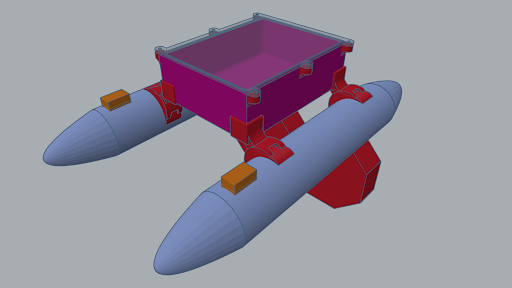
\includegraphics[scale = 0.60]{assets/3d_model_complete.png}
\caption{CAD Model}
\label{fig:3dModelComplete}
\end{figure}

\paragraph{} The study does not consider the potential challenges posed by capsizing due to strong tidal waves or encountering large obstructing objects
            in the ocean. Furthermore, the research does not extensively explore the intricate legal and regulatory frameworks governing unmanned surface 
            drones, instead prioritizing an in-depth examination of the technical aspects related to navigation.

\paragraph{} While the study’s primary focus is on navigation accuracy, the drone is inherently modular(Figure \ref{fig:3dModelComplete}). This modular 
            design enables the replacement of various components to meet the specific requirements of future users, enhancing its versatility and 
            adaptability in different scenarios.

\section{Definition of Terms}
\begin{itemize}
  \item ESP32 -- low-cost, low-power system-on-chip (SoC) microcontrollers designed by Espressif Systems. Widely used in various applications such as 
        IoT (Internet of Things), home automation, wearables, and industrial automation due to its versatility, low cost, and built-in Wi-Fi and Bluetooth
        connectivity. It is commonly programmed using the Arduino IDE or the Espressif IDF (IoT Development Framework).
  \item Shroud -- refers to 3d printed components that covers and protects the propeller from marine debris. Secures brushless motor in place.
  \item Pontoon -- refers to 3d printed components; Provides the drone with enough buoyancy to keep afloat on water.
  \item Enclosure -- refers to 3d printed waterproof containers housing electronic components. 
  \item Bracket -- refers to 3d printed components; Design includes 6 pieces connecting the shroud to the pontoon and the pontoon to the enclosure.
\end{itemize}
\chapter{Review of Related Literature}

The relevance of unmanned sea drones in the modern era is paramount due to their significant role in enhancing maritime 
operations, surveillance, and data collection while minimizing human risk. These autonomous platforms contribute 
significantly to various domains such as environmental monitoring, security, and underwater exploration. Navigational 
systems play a crucial role in the effectiveness of these drones.

Unmanned sea drones employ diverse navigation systems to ensure precise and effective operation. Inertial Navigation 
Systems (INS) utilize accelerometers and gyroscopes to calculate the drone's position by continuously measuring changes 
in velocity and orientation. Acoustic positioning systems leverage underwater sound waves for localization, particularly 
useful in subsea exploration. Additionally, Doppler Velocity Logs (DVL) provide real-time velocity measurements by 
analyzing the echoes of sound waves off the seafloor. These navigation systems collectively contribute to the autonomy 
and adaptability of sea drones in challenging marine environments. However, the magnetometer and GPS stand out as critical 
components due to their roles in determining heading and ensuring accurate global positioning, respectively, forming a 
foundational framework for the seamless navigation of unmanned sea drones.

The incorporation of Global Positioning System (GPS) and magnetometer technologies significantly contributes to improving
autonomous navigation of water drones in maritime environments. This review explores the current state of research and 
developments in utilizing GPS and magnetometers for precise and reliable open sea navigation. Various studies have explored 
the application of GPS technology in drones.

\section{Prior Arts}
\begin{itemize}
\item {\bf An autonomous boat based synthetic aperture} \\
Earlier innovators such as Silva et al. (2007) introduced the Synthetic Aperture Sonar (SAS) system mounted on an 
autonomous boat, specifically designed for mapping and characterizing shallow water environments. Drawing inspiration 
from Synthetic Aperture Radar (SAR), this SAS system leverages the combined processing of transmitted and received 
signals by a moving probe to generate high-resolution images. Unlike traditional narrow-aperture systems, the proposed 
SAS requires simpler hardware and boasts lower operational costs, making it suitable for various applications like 
bottom tomography, river navigability assessments, and infrastructure inspection. The key innovation lies in utilizing 
a floating platform instead of submersed platforms, enabling accurate position and velocity control through satellite 
navigation systems. This, in turn, enhances the quality of sonar images by providing precise motion compensation for 
the synthetic aperture technique. Silva et al. (2007) further emphasize the tight integration of GPS receivers (with 
carrier phase processing), compass, and inertial navigation system (INS) to achieve positioning and attitude accuracy 
below the acoustic wavelength used. This high-precision data feeds into a back-projection algorithm that generates 
absolute-coordinate images, facilitating seamless integration with other geographic information systems. Overall, the 
presented SAS system offers a promising solution for cost-effective and high-resolution mapping of shallow water 
environments, showcasing the potential of integrating advanced navigation technologies with sonar imaging techniques.

\item {\bf Navigation, guidance, and control of an overactuated marine surface vehicle} \\
Further innovations by Đula Nađ, Nikola Mišković, and Filip Mandić (2017) proposed an optimal control strategy based on a 
PID controller to address course keeping during unmanned surface vessel navigation. The authors employ a combination 
of mathematical modeling, data analysis, simulations, and experiments to validate the effectiveness of their approach. 
Their findings demonstrate that the proposed PID control strategy can ensure course stability for unmanned vessels, 
making it a viable solution for autonomous navigation tasks.

\item {\bf Research on a course control strategy for unmanned surface vessel} \\
Recognizing the limitations of traditional GPS and pre-built maps. Luo et al (2021) address the challenge of precise 
course control for unmanned surface vessels (USVs) in dynamic environments by proposing an optimal control strategy 
based on a PID controller. This approach leverages readily available onboard sensors, including odometry, compass 
readings, and occasional landmark measurements, to maintain course stability under the influence of wind, waves, and 
currents. Through a combination of mathematical modeling, simulations, and experiments, Luo et al. (2021) demonstrate 
effectiveness of their PID control method, showcasing its ability to track desired trajectories even in challenging 
scenarios. Their work offers a promising avenue for robust and adaptable navigation of USVs in real-world conditions, 
laying the groundwork for further exploration of sensor fusion and control algorithms for autonomous maritime operations.

\item {\bf Autonomous urban localization and navigation with limited information} \\
Some studies avoided relying on gps entirely, such as Chipka and Campbell(2018) proposing an algorithm for autonomous 
urban navigation with minimal reliance on traditional GPS or pre-built maps. Chipka and Campbell’s (2018) approach 
utilizes an extended Kalman filter to localize the vehicle based on odometry, compass readings, and occasional landmark 
measurements. Navigation is achieved through a compass-based control law. This method demonstrates promising success 
rates in simulated urban environments under various conditions, suggesting a potential pathway for robust autonomous 
driving even in situations where GPS or detailed maps are unavailable. However, further testing and refinement are 
necessary to assess its real-world feasibility and extend its capabilities to handle more complex scenarios.

\item {\bf Autonomous unmanned merchant vessel and its contribution towards the e-navigation implementation: The MUNIN Perspective} \\
On a broader scale;within the European Union, the MUNIN project develops a concept for an unmanned dry bulk carrier 
during deep-sea voyages..introduced by Burmeister et al. (2014), the MUNIN (Maritime Unmanned Navigation through 
Intelligence in Networks)  project, which investigates the feasibility of autonomous unmanned merchant vessels (UAMVs) 
and their potential alignment with the goals of e-Navigation, focusing on enhancing maritime safety and efficiency. 
While initially appearing to conflict with e-Navigation's emphasis on ship-to-shore cooperation, MUNIN effectively 
bridges this divide through its built-in automation features. Firstly, its advanced sensor module surpasses traditional 
systems in both redundancy and accuracy, potentially mitigating human errors in data interpretation and providing more 
dependable navigation information, a fundamental aspect of e-Navigation. Secondly, MUNIN's centralized architecture 
enables real-time monitoring of the vessel's status and surroundings from shore, enabling proactive intervention and 
improved situational awareness, in line with e-Navigation's objective of enhanced shore-based support. Lastly, MUNIN's 
automation directly addresses e-Navigation's goal of reducing seafarer workload by automating routine tasks, thus 
optimizing operational efficiency and easing crew pressure, potentially fostering a safer maritime environment by 
reducing fatigue. Although acknowledging the ongoing research and development needed for UAMV viability, Burmeister 
et al. (2014) conclude that MUNIN's innovative approach provides valuable insights and advancements that could 
significantly enhance the broader e-Navigation framework.
\end{itemize}

\section{Synthesis}
Unmanned sea drones for modern maritime operations offer enhanced surveillance and data collection while minimizing human 
risk. These platforms use various navigation systems like Inertial Navigation Systems (INS), acoustic positioning, and 
Doppler Velocity Logs (DVL), with GPS and magnetometer technologies playing critical roles in precise positioning and 
heading determination. Recent innovations, like the Synthetic Aperture Sonar (SAS) system on autonomous boats, highlight 
the integration of advanced navigation technologies for high-resolution mapping in shallow water environments. 
Additionally, optimal control strategies based on PID controllers are proving effective in ensuring stability and course 
control for unmanned vessels, showcasing advancements in autonomous maritime navigation.

Moreover, initiatives like the MUNIN project explore the feasibility of an autonomous unmanned merchant vessels (UAMVs) 
aligned with e-Navigation objectives, focusing on safety, efficiency, and reduced seafarer workload. By integrating 
advanced sensor modules and centralized automation, these projects aim to enhance navigation accuracy, shore-based 
monitoring, and operational efficiency. Such endeavors address current navigation challenges and pave the way for safer 
maritime operations by reducing human error and fatigue, offering insights into the future of autonomous maritime 
navigation within the broader framework of e-Navigation.

https://doi.org/10.1016/j.arcontrol.2015.08.005  Navigation, guidance, and control of an overactuated marine surface vehicle. 
            Đula Nađ, Nikola Mišković, Filip Mandić

https://doi.org/10.48550/arXiv.1810.04243 Autonomous Urban Localization and Navigation with Limited Information Jordan Chipka, Mark Campbell

https://doi.org/10.1016/j.enavi.2014.12.002  Autonomous Unmanned\\Merchant Vessel and its Contribution towards the e-Navigation Implementation: The MUNIN Perspective

10.1109/OCEANS.2007.4449358 An Autonomous Boat Based Synthetic Aperture Sonar Sergio Rui Silva; Sergio Cunha; Anibal Matos; Nuno Cruz

10.1088/1742-6596/1948/1/012106 Research on a course control strategy for unmanned surface vessel  Zhigang Luo, Tonghui Qian, Xi Ye, Jiahui Huang and Linwen Yu

\begin{table}[h]
  
\begin{tabularx}{\linewidth}{@{} | m{0.15\linewidth} | p{0.06\linewidth} | p{0.06\linewidth} | p{0.06\linewidth} | p{0.06\linewidth} | p{0.06\linewidth} | p{0.12\linewidth} | m{0.21\linewidth} | }
  \hline
 & Prior art 1 & Prior art 2 & Prior art 3 & Prior art 4 & Prior art 5 & Proponent's study & Remarks \\
 \hline
 GPS / Magnetometer based  & \cmark & \xmark & \cmark & \cmark & \cmark & \cmark & Navigation algorithm is highly reliant on GPS / Magnetometer data \\
 \hline
 3d printed materials & \xmark & \xmark & \xmark & \xmark & \xmark & \cmark & Uses PETG (Polyethylene Terephthalate Glycol-Modified), a material known for its water resistance \\
 \hline
 ESP-32 microcontroller & \xmark & \xmark & \xmark & \xmark & \xmark & \cmark & Utilizes an ESP-32 microcontroller \\
 \hline
 Water surface drone & \cmark & \xmark & \xmark & \cmark & \cmark & \cmark & Built for water surface applications \\
 \hline
 Modular design & \xmark & \xmark & \xmark & \xmark & \xmark & \cmark & Modular components are designed to be easily detached or replaced. This allows for quick upgrades, replacements, or modifications \\
 \hline
\end{tabularx}
\label{table:Synthesis}
\end{table}







\chapter{Methodology}

\vspace{-1cm}

This chapter shows the process of designing, testing and troubleshooting tools and equipment, construction and wiring procedure.

Now that the design is in place, the purchase of material will follow, then the construction of the device and lastly the performance,
functionality, and reliability will be tested.

\section{System Design}
\begin{figure}[ht]
  \centering \begin{tikzpicture}
    \node[anchor=north west] (battery) at (0, -0.3) {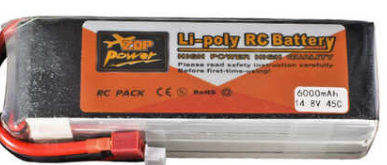
\includegraphics[width=3cm]{assets/battery.png}};
    \node[anchor=north west] (converter) at (5, 0) {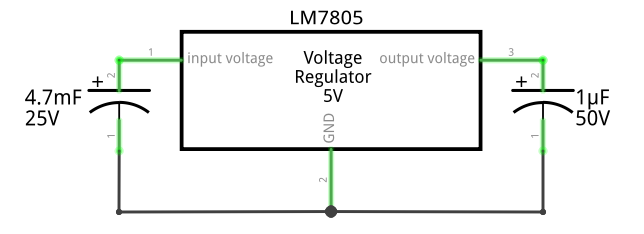
\includegraphics[width=5cm]{assets/converter.png}};
    \node[anchor=north west] (esp32) at (6, -3.5) {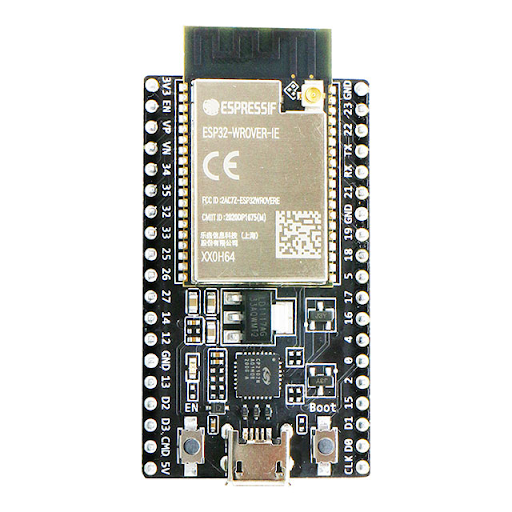
\includegraphics[width=3cm]{assets/esp-32.png}};
    \node[anchor=north west] (magnetometer) at (12, -0.5) {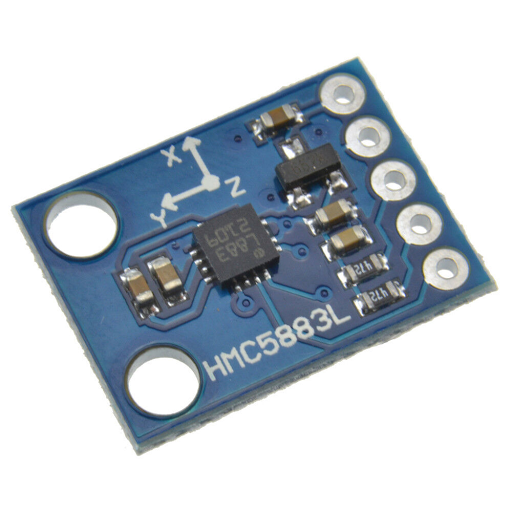
\includegraphics[width=3cm]{assets/magnetometer.png}};
    \node[anchor=north west] (gps) at (12, -6) {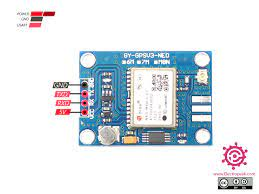
\includegraphics[width=3cm]{assets/gps_module.png}};
    \node[anchor=north west] (esc) at (0, -3.5) {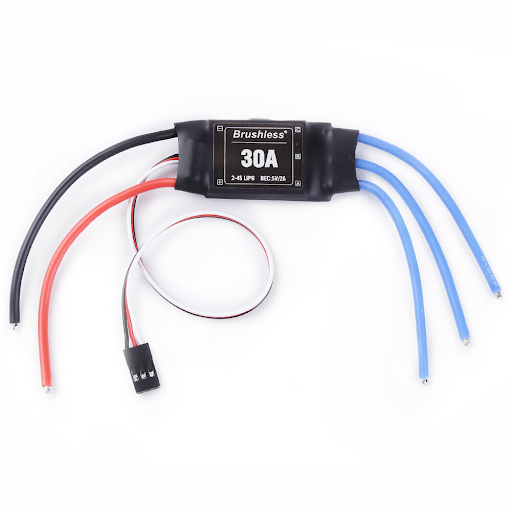
\includegraphics[width=3cm]{assets/esc.png}};
    \node[anchor=north west] (motor) at (3, -8) {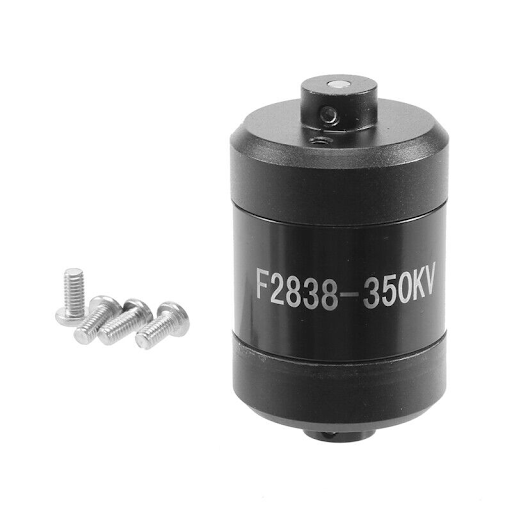
\includegraphics[width=3cm]{assets/motor.png}};
    \node[anchor=north west] (propeller) at (9, -8.2) {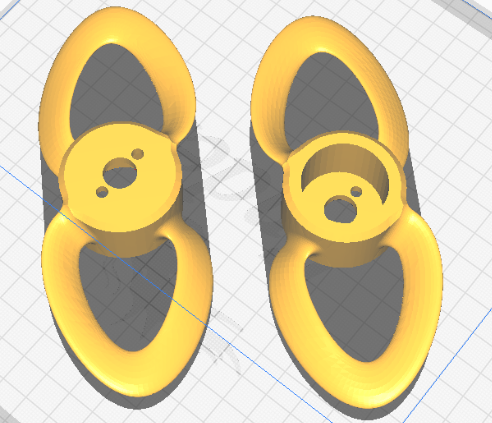
\includegraphics[width=3cm]{assets/propellers.png}};

    \draw[ ->, line width = 1mm, black!70] (battery) to (converter);
    \draw[ ->, line width = 1mm, black!70] (battery) to (esc);
    \draw[ ->, line width = 1mm, black!70] (esp32) to (esc);
    \draw[ <->, line width = 1mm, black!70] (esc) |- (motor);
    \draw[ ->, line width = 1mm, black!70] (motor) to (propeller);
    \draw[ ->, line width = 1mm, black!70] (converter) to (esp32);
    \draw[ <->, line width = 1mm, black!70] (esp32.east) + (0, 0.3) -| (magnetometer.south);
    \draw[ <->, line width = 1mm, black!70] (esp32.east) + (0, -0.2) -| (gps.north);

    % \path[ ->, line width = 1mm, black!70] (esp32.east) + (0, 1) edge [bend left] (magnetometer);
    % \path[ <-, line width = 1mm, black!70] (esp32.east) + (0, 0.5) edge [bend right] (magnetometer.west);
    % \path[ ->, line width = 1mm, black!70] (esp32.east) + (0, -0.5) edge [bend right] (gps);
    % \path[ <-, line width = 1mm, black!70] (esp32.east) + (0, 0) edge [bend left] (gps.west);


  \end{tikzpicture}
  \caption{System Design}
  \label{fig:SystemDesign}
\end{figure}

\pagebreak

% \section{Flowchart}
% \begin{figure}[ht]
% \centering \begin{tikzpicture}
%   [
%   RECT/.style={rectangle, rounded corners, draw=black!60, fill=white!0, very thick, minimum width = 20mm, minimum height = 10mm, align = center},
%   ROUNDEDRECT/.style={rounded rectangle, draw=black!60, fill=white!0, very thick, minimum width = 20mm, minimum height = 10mm},
%   DIAMOND/.style={diamond, draw=black!60, fill=white!0, very thick, minimum width = 10mm, minimum height = 10mm, align = center, aspect = 2, },
%   ]

%   \node[ROUNDEDRECT] (start) {Start};
%   \node[RECT] (switchOn) [below = of start] {Switch on};
%   \node[RECT] (esp32Boot) [right = of switchOn] {ESP-32 boots};
%   \node[RECT] (waitForUserInput) [right = of esp32Boot] {Waiting for user \\ input coordinates};
%   \node[RECT] (coordinatesSupplied) [below = of waitForUserInput] {Coordinates Supplied};
%   \node[RECT] (detectsLocationData) [left = of coordinatesSupplied] {GPS \& magnetometer \\ detects location data};
%   \node[RECT] (droneMoves) [left = of detectsLocationData] {Drone moves to \\ supplied coordinates};
%   \node[RECT] (confirmLoc) [below = of droneMoves] {GPS \& magnetometer \\ confirms location data};
%   \node[] (dummyNode) [below = of detectsLocationData] {};
%   \node[DIAMOND] (doesLocMatch) [below = of dummyNode] {Does drone location match \\ with supplied coordinates?};
%   \node[RECT] (terminate) [below = of doesLocMatch] {Drone terminated};
%   \node[ROUNDEDRECT] (end) [right = of terminate] {End};

%   \draw[ ->, line width = 1mm, black!70] (start.south) to node[] {} (switchOn.north);
%   \draw[ ->, line width = 1mm, black!70] (switchOn.east) to node[] {} (esp32Boot.west);
%   \draw[ ->, line width = 1mm, black!70] (esp32Boot.east) to node[] {} (waitForUserInput.west);
%   \draw[ ->, line width = 1mm, black!70] (waitForUserInput.south) to node[] {} (coordinatesSupplied.north);
%   \draw[ ->, line width = 1mm, black!70] (coordinatesSupplied.west) to node[] {} (detectsLocationData.east);
%   \draw[ ->, line width = 1mm, black!70] (detectsLocationData.west) to node[] {} (droneMoves.east);
%   \draw[ ->, line width = 1mm, black!70] (droneMoves.south) to node[] {} (confirmLoc.north);
%   \draw[ ->, line width = 1mm, black!70] (confirmLoc.south) to node[] {} (doesLocMatch.west);
%   \draw[ ->, line width = 1mm, black!70] (doesLocMatch.north) to node[left] {NO} (detectsLocationData.south);
%   \draw[ ->, line width = 1mm, black!70] (doesLocMatch.south) to node[left] {YES} (terminate.north);
%   \draw[ ->, line width = 1mm, black!70] (terminate.east) to node[] {} (end.west);
% \end{tikzpicture}
% \caption{Flowchart}
% \label{fig:Flowchart}
% \end{figure}

\section{Flowchart}
\begin{figure}[ht]
  \centering \begin{tikzpicture}
    [
      RECT/.style={rectangle, rounded corners, draw=black!60, fill=white!0, very thick, minimum width = 20mm, minimum height = 10mm, align = center},
      ROUNDEDRECT/.style={rounded rectangle, draw=black!60, fill=white!0, very thick, minimum width = 20mm, minimum height = 10mm},
      DIAMOND/.style={diamond, draw=black!60, fill=white!0, very thick, minimum width = 10mm, minimum height = 10mm, align = center, aspect = 3, },
    ]

    \node[ROUNDEDRECT] (start) {Start};
    \node[RECT] (switchOn) [right = of start] {Switch on};
    \node[RECT] (waitForUserInput) [below right = of switchOn] {Waiting for \\ user to provide \\ target coordinates};
    \node[RECT] (waitingForSensor) [below left = of switchOn] {Waiting for GPS and \\ magnetometer modules to \\ process  location and heading};
    \node[DIAMOND] (isUserInputValid) [below = of waitForUserInput] {Is user input \\ valid?};
    \node[DIAMOND] (isSensorDataValid) [below = of waitingForSensor] {Is sensor data \\ valid?};
    \node[RECT] (compute) [below = 5.5cm of switchOn] {Compute distance and \\ bearing to target};
    \node[RECT] (move) [below = of compute] {Drone turns and \\ moves to target};
    \node[DIAMOND] (distance) [below = of move] {Is the distance between \\ the drone and the target within the \\ uncertainty threshold?};
    \node[RECT] (terminate) [below = of distance] {Drone terminated};
    \node[ROUNDEDRECT] (end) [right = of terminate] {End};

    \draw[ ->, line width = 1mm, black!70] (start) to (switchOn);
    \draw[ ->, line width = 1mm, black!70] (switchOn.south) + (3mm, 0) |- (waitForUserInput.west);
    \draw[ ->, line width = 1mm, black!70] (switchOn.south) + (-3mm, 0) |- (waitingForSensor.east);
    \draw[ ->, line width = 1mm, black!70] (waitForUserInput) to (isUserInputValid);
    \draw[ ->, line width = 1mm, black!70] (waitingForSensor) to (isSensorDataValid);
    \draw[ ->, line width = 1mm, black!70] (isSensorDataValid.south)  |- node[below] {Yes} (compute.west);
    \draw[ ->, line width = 1mm, black!70] (isUserInputValid.south) |- node[below] {Yes} (compute.east);
    \draw[ ->, line width = 1mm, black!70] (compute) to (move);
    \draw[ ->, line width = 1mm, black!70] (move) to (distance);
    \draw[ ->, line width = 1mm, black!70] (distance) to node[left] {Yes} (terminate);
    \draw[ ->, line width = 1mm, black!70] (terminate) to (end);
    \draw[ ->, line width = 1mm, black!70] (isSensorDataValid) + (-3, 0) node[below] {No} |- (waitingForSensor.west);
    \draw[ -, line width = 1mm, black!70] (waitingForSensor) + (-3, 0) |- (isSensorDataValid.west);
    \draw[ ->, line width = 1mm, black!70] (isUserInputValid) + (3, 0) node[below] {No} |- (waitForUserInput.east);
    \draw[ -, line width = 1mm, black!70] (waitForUserInput) + (3, 0) |- (isUserInputValid.east);
    \draw[ ->, line width = 1mm, black!70] (distance) + (-6, 0) node[below] {No} |- (move.west);
    \draw[ -, line width = 1mm, black!70] (move) + (-6,0) |- (distance.west);

  \end{tikzpicture}
  \caption{Flowchart}
  \label{fig:Flowchart}
\end{figure}

\section{Navigation algorithm}
\begin{enumerate}
  \item  Get target location \tLoc from the user

        \tLoc is acquired from the user by specifying its geo-coordinates in the \emph{Latitude-Longitude} format. Latitude values denote the angular distance relative
        to the equator, with positive values indicating locations north of the equator and negative values indicating locations south of the equator. Similarly, Longitude values
        represent the angular distance east or west of the Prime Meridian, with positive values corresponding to western locations and negative values signifying eastern locations.
        \emph{Both Latitude and Longitude should be specified as decimal degrees.}

  \item  Get current location \cLoc and current heading \heading from GPS and magnetometer modules

        \cLoc is acquired from the Global Positioning System (GPS) module. The module transmits NMEA sentences (refer to Section X.X todo for a detailed
        explanation) to the ESP32 microcontroller.  Of these sentences, the GPGLL sentence is specifically processed to extract the latitude, north/south (N/S) indicator, longitude,
        east/west (E/W) indicator, and validity status.  The latitude and longitude values are converted from the degrees-minutes-decimal minutes format (dddmm.mmmm)
        to decimal degrees for further calculations.  Subsequently, the N/S and E/W indicators are used to determine the correct sign (positive or negative) for the extracted
        latitude and longitude values.

        In contrast, \heading is calculated based on the \emph X and \emph Y values obtained from the magnetometer module.
        This value represents the device's orientation relative to magnetic north. The calculation of \heading requires the declination angle \decAngle which is itself derived from the
        longitude component of the current location, \cLoc. The declination correction accounts for the difference between magnetic north and true geographic north.  This correction is
        applied to the magnetic heading which is an azimuth value between 0 and 359 degrees, to obtain a value that represents the device's orientation relative to
        true north.
        $$ \theta_c = \atantwo(y, x) + \frac{180}{\pi} + (\underbrace{0.015}_{\mathclap {\text{\hspace{+3.5cm} constant used to approximate angle of declination}}} * X_c^\lambda) + 1 $$

        A specific function is then used to ensure the resulting value remains within the 0 to 359 degree range and avoids overflow errors.


  \item Get the difference between between the longitude \longDiff and latitude \latDiff components of \cLoc and \tLoc
        \begin{align*}
          \lambda & = X_c^\lambda - X_t^\lambda \\
          \phi    & = X_c^\phi - X_t^\phi
        \end{align*}

  \item Get distance \distance between \cLoc and \tLoc

        Due to the Earth's oblateness, getting the distance between two geographic coordinates presents complexities. The conversion factor required for accurate
        transformation varies depending on the specific location on the Earth's surface. To address this, we will leverage an approximate formula used in the source
        code of CSGNetwork.com's length of a degree of latitude and longitude calculator\cite{sourcecode}. This formula was further explored in an answer in a forum post in the
        Geographic Information Systems Stack Exchange website\cite{forum} indicating that it was derived from the WGS84 ellipsoidal Earth model.

        $$ \phi_m = \frac{X_c^\phi + X_t^\phi}{2} $$
        \begin{align*}
          \phi_d = \text{ meters per degree in } \phi       & = 111132.92 \; - \; 559.82\cos2{\phi_m}       \\ & \quad +  \; 1.175cos4\phi_m \; - \; 0.0023\cos6\phi_m \\ \\
          \lambda_d = \text{ meters per degree in } \lambda & = 111412.84\cos\phi_m \; - \; 93.5\cos3\phi_m \\ & \quad + \; 0.118\cos5\phi_m
        \end{align*}

        To find the distance in meters, we will apply the Pythagorean Theorem.

        $$ \Delta = \sqrt{{(\phi_d)}^2 + {(\lambda_d)}^2} $$

  \item Get target bearing \bearing from \cLoc to \tLoc

        Assuming that the \cLoc and \tLoc is in a two-dimensional Cartesian plane centered at \cLoc, we determine \bearing using the \emph{atan} function and
        quadrant-specific adjustments. The \emph{arctangent}, expressed as $\arctan(\frac{\lambda}{\phi})$ calculates the fundamental inclination angle. To account for the
        varying quadrants and to ensure an accurate directional representation from the origin, corrective terms of 180\degrees or 360\degrees are incorporated based
        on the signs of \longDiff and \latDiff. This simple approach offers a robust and computationally efficient method for calculating azimuths within the assumed two-dimensional
        spatial framework.

        $$ \theta_t = \begin{cases}
            \arctan(\frac{\lambda}{\phi})       & \text{if } \lambda > 0 \text{ and } \phi > 0 \rightarrow \text{quadrant 1} \\
            \arctan(\frac{\lambda}{\phi}) + 180 & \text{if } \lambda > 0 \text{ and } \phi < 0 \rightarrow \text{quadrant 2} \\
            \arctan(\frac{\lambda}{\phi}) + 180 & \text{if } \lambda < 0 \text{ and } \phi < 0 \rightarrow \text{quadrant 3} \\
            \arctan(\frac{\lambda}{\phi}) + 360 & \text{if } \lambda < 0 \text{ and } \phi > 0 \rightarrow \text{quadrant 4} \\
          \end{cases} $$

  \item Calculate relative bearing \rBearing between \bearing and \heading

        The raw relative bearing $\boldsymbol{\delta}$ is subsequently calculated by subtracting the measured heading \heading from the target bearing \bearing.

        $$ \delta = \theta_c - \theta_t $$

        To constrain \rBearing within the range of -180\degrees \space to 180\degrees, a correction step is implemented to the raw relative bearing. If the absolute value of \rawBearing exceeds
        180\degrees, the absolute value \rawBearing is subtracted from 360\degrees. This ensures that \rBearing remains as close to zero as possible.
        A minimal relative bearing value translates to the smallest required turning angle.

        $$ \theta = \begin{cases}
            \delta         & \text{if } |\delta| \leq 180 \\
            360 - |\delta| & \text{if } |\delta| > 180
          \end{cases} $$

  \item Differential thrust for yaw control
  
        To achieve yaw (turn) maneuvers, the relative bearing, \rBearing, dictates the power distribution between the designated motors. Positive \rBearing signifies a turn
        towards the port side (left), while negative \rBearing corresponds to a starboard (right) turn.

        To generate yaw torque, one motor experiences a reduction in thrust while the opposing motor stays at the maximum thrust. For a port turn, the port motor's thrust is reduced
        and the starboard motor's thrust stays at the maximum. Conversely, a starboard turn necessitates the opposite configuration.

        To minimize the duration of reduced thrust on a single motor and reduce transient effects, a damping value function is implemented. When the relative bearing is within a predefined
        tolerance zone of 5\degrees$\pm$, both motors operate at full capacity, effectively maintaining straight travel.

        For relative bearings exceeding the tolerance thresholds, the thrust of the appropriate motor is reduced linearly. In a scenario requiring a full port turn, the port motor's thrust 
        would be linearly reduced to zero while the starboard motor maintains maximum thrust. Conversely, a full starboard turn would involve linearly scaling the starboard motor's thrust to 
        zero while maintaining maximum thrust on the port motor.

        When the drone's distance to the target, designated by \distance, is within the \emph{uncertainty threshold}, both of the motors would provide no thrust. If \distance has increased to 
        above the \emph{uncertainty threshold} due to drift, then the algorithm will loop back up again and try to correct the drift.
\end{enumerate}

When the distance to the target, \distance, falls within the \emph{uncertainty threshold}, both motors are commanded to produce zero thrust as the target is sufficiently close. However,
if the distance exceeds the \emph{uncertainty threshold} due to factors such as environment disturbance or drift, the control algorithm iterates back to the beginning and initiates corrective
actions to re-establish accurate positioning relative to the target.

\section{Construction Procedure}

\section{Testing and Evaluation}

\section{Sources of Data}

\section{Project Components and Materials}

\section{Instruments}


\end{document}
